\section{Network}

Fig.~\ref{fig:network-arch} shows an abstraction of a typical RSS3 Network architecture. In short, an RSS3 file is served by a subgroup which consists of several SNs. A subgroup is managed by GIs and forwards client requests to its SNs. A GI consists of: 1) a set of relay nodes to assist in routing; 2) a set of archive modules to archive the network for failure recovery in the event of a large-scale network crash.

\subsection{Decentralized Autonomous Organization (DAO)}

DAO is responsible for governing the followings:
\begin{multicols}{2}
    \begin{itemize}
        \item GI and SN Elections
        \item RSS3 Files limit per SN
        \item \mbox{DKG key fragments} threshold
        \item Subgroup scaling
        \item Module upgrade
        \item Incentive Management
        \item ER Duration
    \end{itemize}
\end{multicols}

\subsubsection{Election Mechanism}

GIs and SNs are elected members that support the network's essential operations. There are entry requirements for candidates to be qualified for participating in an election: These requirements may include hardware and staking set by DAO. GI elections are held less frequently than SN elections. Each election may produce an abundance of nodes and only the required number of nodes will be immediately placed into work. $S=\{s_1, s_2,...,s_{\mathcal{S}}\}$ is the set of all SNs, whose number is $\mathcal{S}$. $G=\{g_1, g_2, ..., g_{\mathcal{G}}\}$ and is denoted as the set of all GIs, whose number is $\mathcal{G}$.

To further strengthen the network, a waiting list ${S'}$ is in place to host idle elected SNs as backup. DAO sets a MOC warning level, $\mathcal{MOC}(m)$, backup SNs will be commissioned once the number of functioning SNs falls below $\mathcal{MOC}(m)$ to avoid subgroup failures.

\subsubsection{Module Upgrade}

WebAssembly modules are used by SNs for indexing to ensure that indexing results are cross-platform deterministic. Modules can be contributed by the network participants and are governed by DAO.

\subsubsection{Subgroup Scaling}

During each ER, DAO may dynamically adjust the size of subgroups, denoted $\mathcal{N}$, to meet the network's needs while maintaining a sufficient level of decentralization. Hence, the number of subgroups $\mathcal{Y}=\lceil\frac{\mathcal{S}}{\mathcal{N}}\rceil$ is dynamic and decided by $\mathcal{S}$ and $\mathcal{N}$. This adjustment predominately ensures the network's performance and stability.

\subsubsection{Incentive Management}

Within each ER, DAO may dynamically adjust the incentive ratio for network participants. Incentive is calculated based on multiple factors, including verified contributions from GIs and SNs on chain , as shown in Fig.~\ref{fig:hbc-proof}. All incentives are distributed from an incentive pool described in Sec.~\ref{subsec:{Incentive Pool}}. A staking pool is governed by DAO, each candidate will be notified of the level staking required to participate in the election. Slashing occurs when an elected node failed to meet its obligations outlined in Sec.~\ref{sec:{Network}}.

\begin{figure}[tb!]
    \centering
    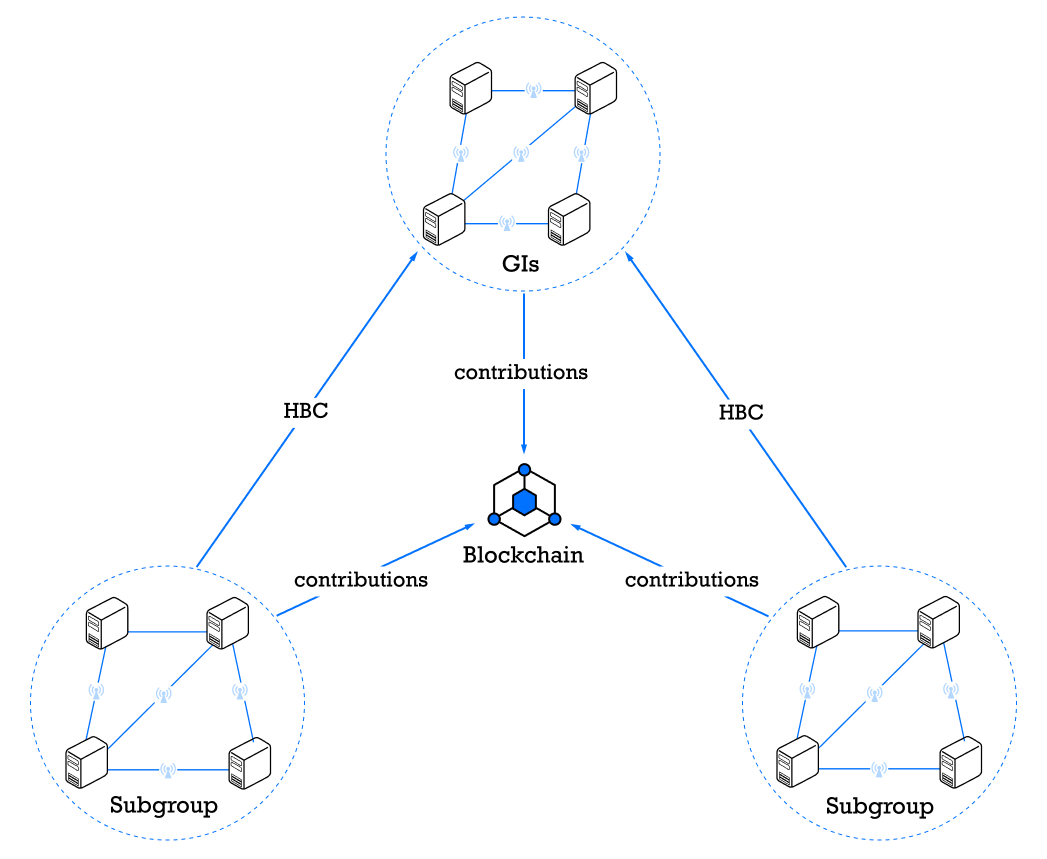
\includegraphics[width=\columnwidth]{figures/hbc.jpg}
    \caption{HBC and Proof on chain.}
    \label{fig:hbc-proof}
\end{figure}

\subsection{Global Indexer (GI)}

GIs are elected by the network participants through DAO. A GI has three major responsibilities: Scalable Dynamic Grouping, Routing and Heartbeat Checking. GIs are assisted by functional nodes listed in Table~\ref{table:glossary}, the details are elaborated below in this section.

A GI at any time may announce its intention to quit the network and gracefully do so at the end of the current ER without slashing. If the MOC is reached, DAO will hold a new round of GI election immediately to avoid a potential network failure.

\subsubsection{Scalable Dynamic Grouping (SDG)}

At the beginning of each ER, SNs are shuffled into different subgroups $S_z;\forall z \in [1,\mathcal{Y}]$ abiding by a modern Byzantine fault tolerant (BFT) algorithm\cite{castro2002Practical,lamport1982Byzantine,badger-bft, tendermint}, to fundamentally prevent collusion attacks. The organization of subgroups is periodically shuffled by GIs through a consent structure, and broadcast to SNs to initiate the re-organization. Subgroups are scalable to incorporate newly available SNs to extend their capability, up to the limit $\mathcal{N}$ imposed by DAO. The number of subgroups is dynamically scaled by the network's existing load based on the strategy agreed by DAO.


To further elaborate on how a consent structure is agreed to, SDG begins with a random number calculated by collecting signatures from GIs. Based on the distributed key generation protocol Ped-DKG\cite{dkg} and Threshold BLS Signatures\cite{bls}, each GI contributes a key fragment as one constituent to form a public and private key pair, the random number is then derived from all the signatures collected, where the DKG key fragments threshold set by DAO is met to guarantee security. SDG proceeds to shuffle SNs and forms a new subgroup structure until not a single subgroup contains $\mathcal{P}$ SNs from the previous ER:
\begin{equation}
\label{BFT}
\mathcal{P}=\lfloor\frac{\mathcal{N}-1}{3}\rfloor; \forall \mathcal{N} \in \mathbb{N}^+
\end{equation}

GI members will be dynamic, allowing GI to join and leave at the next ER. The change of GI members will affect the generation of distributed random numbers, as it depends on the key fragmentation of each GI member. Proactive secret sharing protocol is adopted\cite{pss,pss2}, which allows a group of GI members to keep the shared key and dynamically transfer the key fragments among different GI members. So as to achieve such a result, that the keys shared among the GI member group fragments are saved in different groups.

In order to minimize the chance of node collusions, at the $e^{th}$ ER, GIs ensure that during SDG:

\begin{itemize}
    \item The subgroup set $\{S_z\}$ is generated by SDG, feeding all SNs as input based on parameter $\mathcal{P}$ and $\eta^e \in \mathbb{N}^+$:
        \begin{align}
            \{S^e_z\} = \mathcal{SDG}(<\{s^{e}_1, s^{e}_2,...,s^{e}_\mathcal{S}\}>;\mathcal{P},\eta^e, \mathcal{Y}^e)
        \end{align}
    \item The intersection of all subgroups is an empty set:
        \begin{align}
            % \bigcap_1^{\mathcal{Y}^e} S^e = S^e_1 \cap S^e_2 \cap ... \cap S^e_{\mathcal{Y}^e}= \varnothing
            \bigcap_{z=1}^{\mathcal{Y}^e} S^e_z = \varnothing
        \end{align}
    \item The union of all subgroups is the set of all SNs:
        \begin{align}
            % \bigcup_1^{\mathcal{Y}^e} S^e = \{s^{e}_1, s^{e}_2,...,s^{e}_\mathcal{S}\} = S^e
            \bigcup_{z=1}^{\mathcal{Y}^e} S^e_z = S^e
        \end{align}
    \item Any $\mathcal{P}$ SNs in the $z^{th}$ subgroup $S^e_z$ will not be grouped into the same subgroup in $\eta^e$ consecutive ERs:
        \begin{align}
            &|S^e_z \cap S^{e-j}_v| < \mathcal{P}; \forall z,v \in [1,\mathcal{Y}^e], \forall j \in [1,\eta^e] \\
            &s^e_{z,i} \notin S^{e-j}_z;\forall s^{e}_{z,i} \in S^e_z, \forall i \in [1, |S^e_z|]
        \end{align}
\end{itemize}

where $S^e_z$ denotes the set of SNs in the $z^{th}$ subgroup at the $e^{th}$ ER, $s^e_{z,i}$ refers to the $i^{th}$ SN in the $z^{th}$ subgroup at the $e^{th}$ ER, and both $\mathcal{P}$ and $\eta$ are set by DAO. More details regarding the procedure of SDG are presented in Algorithm~\ref{alg:sdg}.

\begin{algorithm}[tb!]
\caption{$\mathcal{SDG}(<S^e>; \mathcal{P}, \eta^e, \mathcal{Y}^e)$}
\label{alg:sdg}
    \begin{algorithmic}[1]
        \WHILE{$\mathcal{SDG} \leftarrow fail$}
            \FOR{$s^e_{z,i} \in S^e_z;z \in [1,\mathcal{Y}^e]; i \in [1, |S^e_z|]$}
                \FOR{$j \in [1, \eta^e]$}
                    \IF{$(| S^e_z \cap S^{e-j}_v| < \mathcal{P}) \land (s^e_{z,i} \notin S^{e-j}_z)$}
                        \STATE $\mathcal{SDG} \leftarrow success$
                        \RETURN $\{S^e_z\}$
                    \ENDIF
                \ENDFOR
            \ENDFOR
        \ENDWHILE
    \end{algorithmic} 
\end{algorithm}

\subsubsection{Robust Routing}

GIs maintain a routing table, which follows the SDG at each ER. GIs are walled by a set of RNs. Following the routing table, RNs accept and forward user requests to the corresponding subgroup.

\subsubsection{Heartbeat Checking (HBC)}
GIs make the best effort to guarantee a subgroup's MOC, see Eqn. \ref{eqn.Critical} and \ref{eqn.MinimumNodes}, where \(n\) denotes the number of SNs, $\mathcal{W}_s$ is set by DAO, satisfying $\mathcal{C}<\mathcal{W}_s<\mathcal{N}$, and $\mathcal{C}$ is the minimum number of SNs supporting the system's MOC. Once the warning level is breached, GI will start enlisting SNs from the waiting list ${S'}$. Once the critical level is breached, GI will immediately start a new round of partial SDG to avoid a potential subgroup failure. A partial SDG re-balances current subgroup in order to satisfy MOC without interrupting network operations.

\begin{align}
\mathcal{C} &= \lceil \frac{2\mathcal{N}}{3} \rceil \label{eqn.Critical}\\
\mathcal{MOC}(n) &= \begin{cases}
                  safe,     & if \ n > \mathcal{W}_s;\\
                  warning,  & if \ \mathcal{C} < n\le \mathcal{W}_s; \\
        	      critical, & if \ n \le \mathcal{C}.
        		   \end{cases}
\label{eqn.MinimumNodes}
\end{align}

Furthermore, a new GI election would start immediately as the number of GIs, namely $m$, reaches the warning level $\mathcal{W}_g$, which is set by DAO. See Eqn.~\ref{eqn:moc_gi}.
\begin{equation}
\mathcal{MOC}(m) = \begin{cases}
                  safe,     & if \ m > \mathcal{W}_g;\\
                  warning,  & if \ m \le \mathcal{W}_g; \\
        		   \end{cases}
\label{eqn:moc_gi}
\end{equation}

\subsection{Serving Node (SN)}

Fig.~\ref{fig:sn-arch} illustrates the internal architecture of a subgroup.

A list of elected SNs, along with their permitted serving ERs, is governed by DAO. Candidates ${s'}$ who were elected but not commissioned are placed on a waiting list ${S'}$, see Sec.~\ref{subsubsec:{Election Mechanism}}. 

\begin{figure}[tb!]
    \centering
    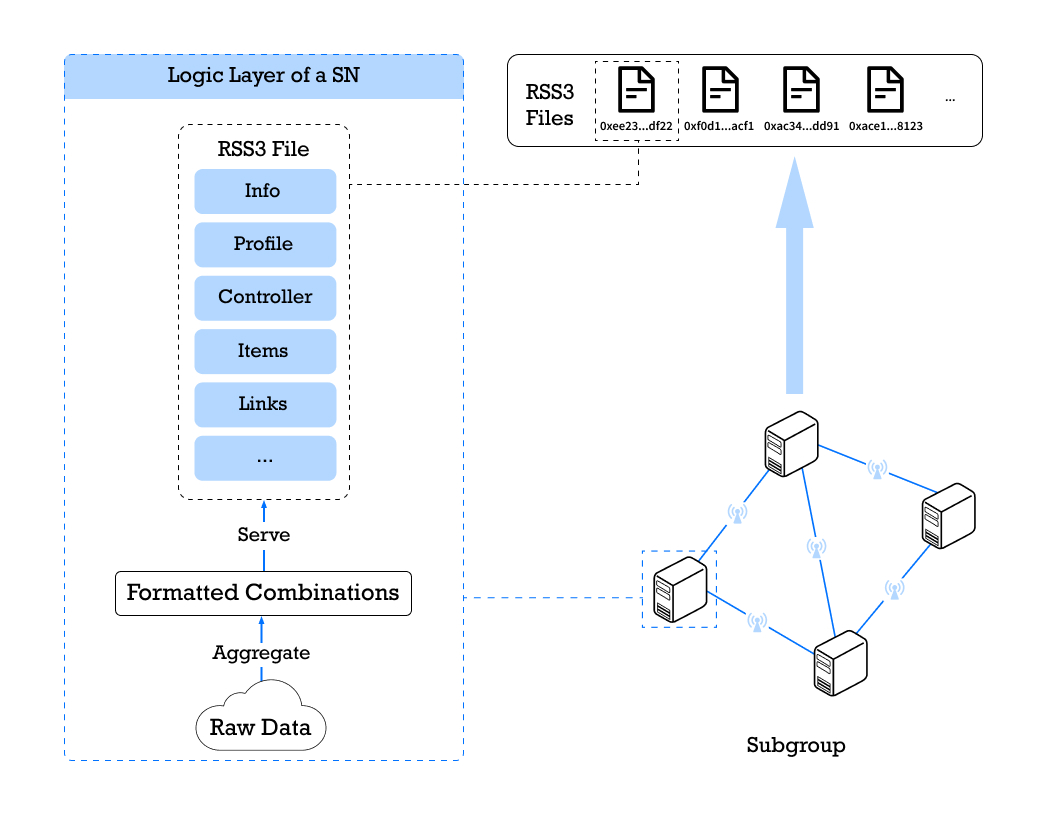
\includegraphics[width=\columnwidth]{figures/sn-arch.jpg}
    \caption{The internal architecture of a subgroup.}
    \label{fig:sn-arch}
\end{figure}

An exit mechanism is in place to permit the departure of SNs from their subgroups during an ER without slashing: 1) the departure must be broadcast to the subgroup to confirm that the MOC level, denoted $\mathcal{C}$, is maintained; 2) the departure must not occur consecutively within $\eta$ ERs, where $\eta$ is set by DAO.

\subsubsection{Information Aggregation}

RSS3 files of the entire network are distributed across many subgroups. Each SN serves a number of RSS3 files and handles the requests targeted at these files according to the standard specifications. SNs use WebAssembly modules for indexing, which ensures that indexing results are cross-platform deterministic. SNs begin with indexing data from verified accounts, perform permission and ownership verification, and eventually generate the instance's activity feeds.


\begin{algorithm}[tb!]
\caption{An algorithmic abstraction of an ER in the RSS3 Network.}
\label{alg:RSS3Network}
    \begin{algorithmic}[1]
    \FOR{each ER $e \in [0,\infty)$}
        % \item[]

        \STATE init. $\mathcal{G}^e, \mathcal{S}^e, \mathcal{N}^e, \mathcal{W}^e_s, \mathcal{W}^e_g, \eta^e$ by DAO
        \STATE $\mathcal{Y}^e \leftarrow \frac{\mathcal{S}^e}{\mathcal{N}^e}$
        \IF{election}
            \STATE $G^e \leftarrow \{{g}^e_1, {g}^e_2, ..., {g}^e_{\mathcal{G}^e}\}$ % GI nodes set
        \ENDIF
        
        \STATE $\{S^e_z\} \leftarrow \mathcal{SDG}(<\{s^{e}_1, s^{e}_2,...,s^{e}_\mathcal{S}\}>;\mathcal{P},\eta^e, \mathcal{Y}^e)$

        \item[]

        \FOR{$S^e_z \in \{S^e_1, S^e_2,...,S^e_{\mathcal{Y}^e}\}$}
            \STATE $n \leftarrow |S^e_z|$
            \Switch{$\mathcal{MOC}(n)$}
                \Case{$n > \mathcal{W}^e_s$}
                    \STATE pass
                \EndCase
                \Case{$\mathcal{C} < n\le \mathcal{W}^e_s$}
                    \STATE $S^e_z \leftarrow {s'}^e_k; \forall {s'}^e_k \in {S'}^e$
                \EndCase
                \Case{$n \le \mathcal{C}$}
                    \STATE ${S'}^e \leftarrow s^e_l; \forall s^e_l \in \{\complement_{S^e}{S^e_z}\}$
                    \STATE $\hat{S}^e_z \leftarrow \mathcal{SDG}(<{S'}^e>;\mathcal{P},\eta^e, \mathcal{Y}^e)$
                \EndCase
        \ENDFOR
        \item[]

        \STATE $m \leftarrow |G^e|$
        \Switch{$\mathcal{MOC}(m)$}
            \Case{$m > \mathcal{W}^e_g$}
                \STATE pass
            \EndCase
            \Case{$m \le \mathcal{W}^e_g$}
                \STATE $\hat{G}^e \leftarrow \{\hat{g}^e_1, \hat{g}^e_2, ..., \hat{g}^e_{\mathcal{G}^e}\}$
            \EndCase
        
        
        \item[]

        \STATE consensus number $c\leftarrow0$
        \FOR{$g^e_z \in G^e \lor \hat{g}^e_z \in \hat{G}^e$}
            \IF{$g^e_z \lor \hat{g}^e_z$ agrees}
                \STATE $c\leftarrow c+1$
            \ENDIF
        \ENDFOR
        \IF{$c > \lceil\frac{2\mathcal{G}^e}{3}\rceil$}
            \STATE submit proof on chain
        \ENDIF

        \item[]
        
        \STATE init. and adjust $P$ and $\Phi$ by DAO
        \STATE $P \leftarrow \{p_{nod}, p_{dev}, p_{cre}, p_{con}, p_{dao}\}$
        \STATE $\Phi \leftarrow \{\alpha,\beta,\gamma,\delta,\epsilon\}$
        \FOR{$i \in [1,5]$}
            \STATE $P_i \leftarrow \Phi_i \mathcal{I}$
        \ENDFOR

    \ENDFOR
    \end{algorithmic} 
\end{algorithm}

\subsubsection{Collaboration}

SNs collaborate within of the same subgroup to reach an internal consensus for finalizing the content of RSS3 Files and acknowledging peer contributions for HBC. SNs are obligated to broadcast their HBC back to GIs for next ER's preparation and incentive distribution. Absence from this process will result in the following consequences for the absentees : 1) to be removed from the incentivization of this ER; 2) removed from the next ER's SDG; 3) to be slashed. At the end of each ER, those HBCs are packed and reported on chain, as the proof of contributions.
% \\

Algorithm~\ref{alg:RSS3Network} shows the algorithmic abstraction of an ER in the RSS3 Network, and Fig.~\ref{fig:flow} illustrates the flow of the abstraction.

{
\begin{figure}[tb!]
    \centering
    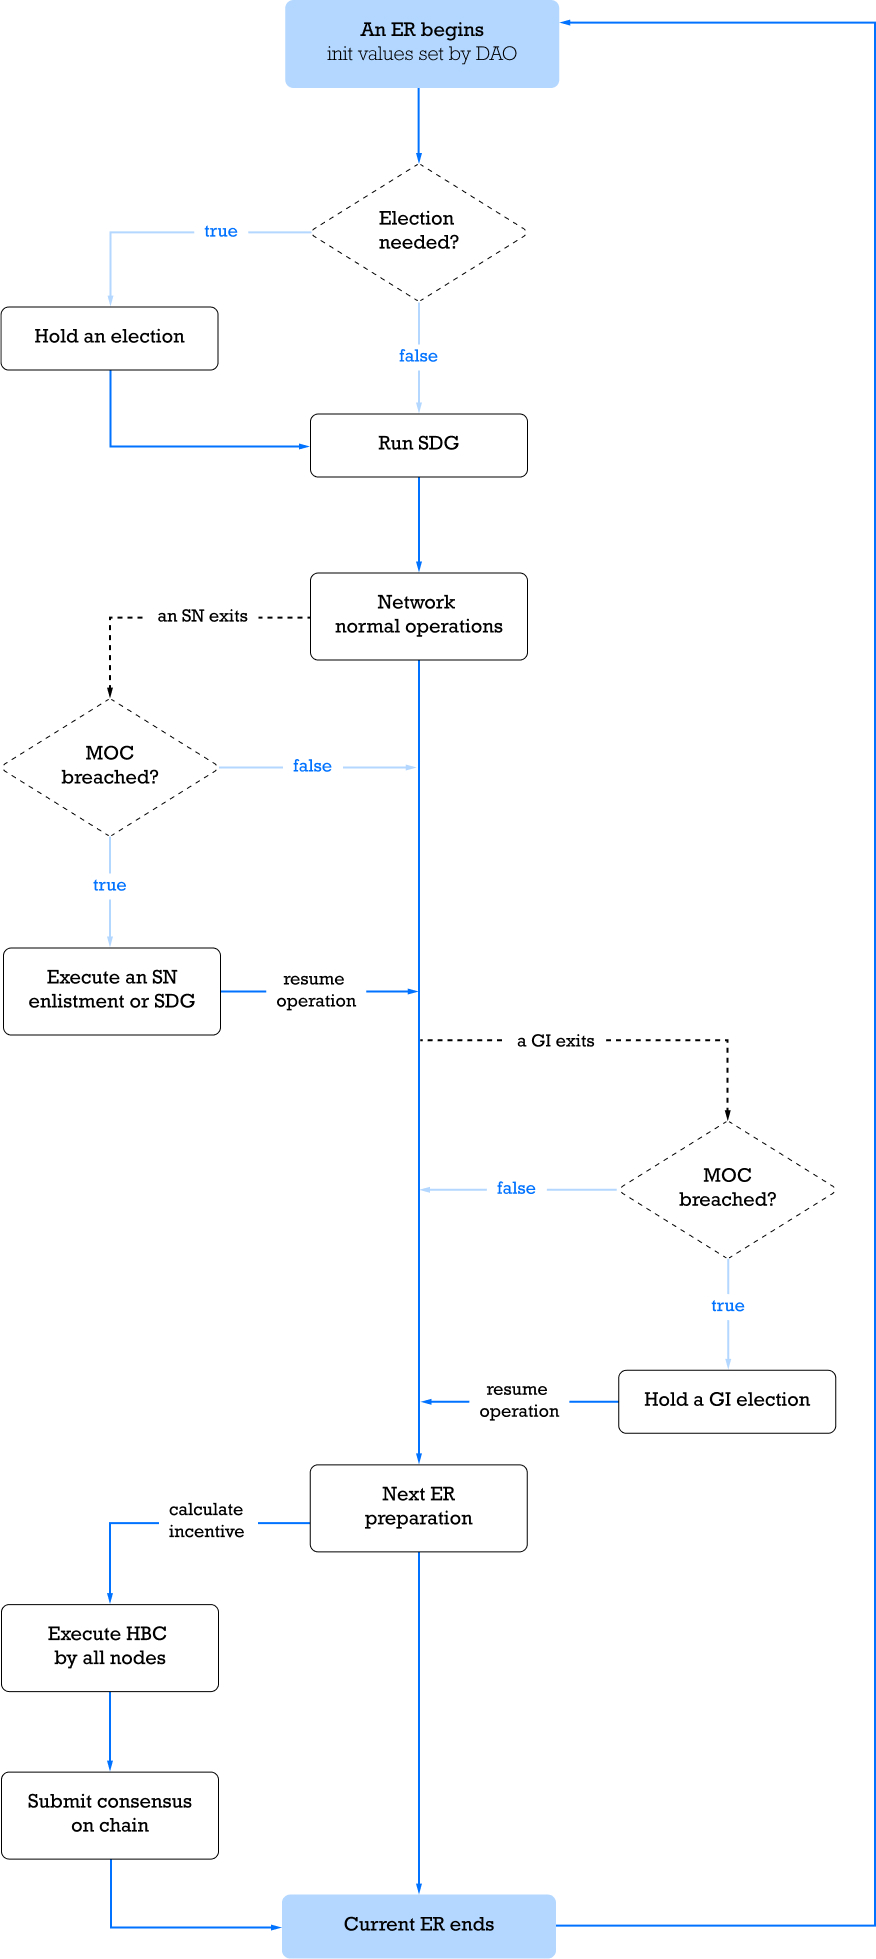
\includegraphics[width=\columnwidth]{figures/flow.jpg}
    \caption{A flowchart illustrating the abstraction of an ER in the RSS3 Network.}
    \label{fig:flow}
\end{figure}
% \setlength{\belowskip}{-10pt}
}